\documentclass[11pt]{article}

\usepackage[margin=1in]{geometry}
\usepackage{amsmath}
\usepackage{amssymb}
\usepackage{array}
\usepackage{booktabs}
\usepackage{graphicx}
\usepackage{hyperref}
\usepackage{xcolor}
\usepackage{url}

\graphicspath{{../figures/}{figures/}}

\title{Online-Consistent Event-Conditioned Guidance for SAT Solving}
\author{Anonymous Authors}
\date{}

\begin{document}

\maketitle

\begin{abstract}
Learning-guided SAT solvers face a practical tension. One-shot neural guidance is efficient because the neural model is queried only once before search, but it remains open-loop: it cannot react to what the CDCL solver observes during search. Fully dynamic neural branching can condition on solver state, but frequent neural calls inside the branching loop introduce substantial wall-clock overhead and can harm complete-solver reliability. This paper studies a conservative middle ground: low-frequency CDCL event traces are used to decide whether neural feedback should be activated at all.

We propose an Online-Consistent Selector for event-conditioned SAT guidance. The solver first obtains a one-shot neural guidance prior, runs short warmup probes to collect CDCL events, and then applies a conservative risk/recovery controller to choose between the one-shot path and an event-adapted guidance path. The selector is trained from same-evidence branch counterfactuals and is designed to recover hard or timeout instances while avoiding lost solutions and unnecessary slowdowns. As an ablation, we further study a guarded Local Boundary Correction that reopens a small set of over-conservative selector decisions under a candidate manifest.

On 200 held-out 3SAT-400 instances, the Online-Consistent Selector improves the one-shot neural guidance baseline from 50/200 to 56/200 solved instances and reduces mean wall-clock time from 47.752s to 46.222s. Local Boundary Correction preserves the 56/200 solved count but further reduces mean time to 45.498s, supporting its role as a boundary repair ablation rather than a separate primary method. These results suggest that sparse, event-conditioned, risk-controlled intervention is a practical way to use solver feedback without turning SAT solving into per-branching neural inference.
\end{abstract}

\section{Introduction}

Modern CDCL SAT solvers are highly optimized, and even useful learned guidance can be harmful if it is inserted at the wrong point in the solving loop. One-shot neural guidance is attractive because it queries a graph neural network once before search and then lets the solver run normally, but this efficiency comes with an open-loop limitation: the guidance cannot react to conflicts, propagations, learnt clauses, or activity patterns observed during search. Dynamic neural branching can use such solver state, but frequent neural inference inside the branching loop creates wall-clock overhead and can introduce reliability risks for a complete solver. This paper asks whether solver feedback can be used more selectively: not to replace the branching heuristic at every decision, but to decide when neural feedback should be activated at all.

The central difficulty is asymmetric risk. A learned adapter can recover hard instances or reduce long-tail runtime, but it can also lose instances that the base one-shot path solves or slow easy instances enough to erase the gains. Therefore, a useful feedback mechanism should not simply maximize adapter usage. It should intervene only when observed solver evidence suggests meaningful recovery potential and low slowdown or lost-solution risk.

We study this problem in the setting of RLAF-style one-shot SAT guidance \cite{rlaf}. The solver first predicts a neural guidance prior from the CNF graph. It then performs low-budget warmup probes under that prior and collects CDCL event traces. These traces provide variable-level and graph-level evidence about the actual search trajectory. An Online-Consistent Selector uses this evidence to decide whether to run the final solve with event-adapted guidance or with the safer one-shot guidance.

Our main contribution is not a more complex branching model. Instead, it is a conservative control layer around neural feedback:
\begin{enumerate}
    \item We propose an event-conditioned online selector that uses real CDCL event traces to decide whether neural feedback should be activated.
    \item We introduce conservative risk control for neural SAT guidance, separating recovery potential from slowdown and lost-solution risk.
    \item We present guarded Local Boundary Correction, a constrained boundary-repair ablation for over-conservative selector errors.
\end{enumerate}

\section{Related Work}

\paragraph{Learning-guided SAT solving.}
Neural SAT methods inject learned predictions into complete solvers in several ways. NeuroSAT showed that message passing can learn useful SAT representations from satisfiability supervision \cite{neurosat}. NeuroCore used neural unsat-core predictions to guide high-performance SAT solvers through variable activity \cite{neurocore}. Graph-Q-SAT studied reinforcement learning for GNN-based branching heuristics \cite{graphqsat}. NeuroBack and RLAF emphasize practical low-frequency guidance by predicting backbones, phases, weights, or polarities before search rather than querying a neural model at every decision \cite{neuroback,rlaf}. Our work follows this practical line but differs in one key respect: the guidance decision is not purely static. We use the one-shot neural guidance prior to collect warmup CDCL event evidence, then decide conservatively whether event-conditioned feedback should be activated for the final solve.

\paragraph{Solver-state and trace-based learning.}
Several systems use solver-internal information rather than only static CNF structure. Graph-Q-SAT and RDC-SAT condition learned decisions on evolving solver states \cite{graphqsat,rdcsat}, while trace-supervised systems such as ImitSAT and NeuroSelect show that CDCL traces, clauses, activities, and other solver artifacts can provide useful learning signals \cite{imitsat,neuroselect}. Our use of solver feedback is narrower. We do not learn a full branching policy, splitting policy, or clause-deletion policy. Instead, we collect event traces at configured intervention points and use them for a single risk-controlled activation decision.

\paragraph{Risk-controlled neural intervention.}
Portfolio and per-instance algorithm selection have long been important in SAT solving \cite{satzilla,kotthoff}. Our selector is narrower than a solver portfolio: it decides whether to activate neural feedback for a given instance, not which solver to run. This decision is still risk-sensitive. A heuristic that improves a few hard instances can be undesirable if it loses solutions or slows many easy instances. We therefore separate recovery evidence from slowdown and lost-solution risk, and report solved count, wall-clock mean, and per-instance behavior rather than a single aggregate metric.

\paragraph{Event-conditioned identity.}
Static message-passing GNNs are limited by neighborhood aggregation, often analyzed through the Weisfeiler-Leman hierarchy \cite{gnnpowerful,morriswl}. SAT instances can contain variables that are structurally similar in the CNF graph but behave differently once CDCL search begins. CDCL event traces provide search-induced distinctions through decisions, propagations, conflicts, learnt-literal occurrences, and activity. We do not claim that these traces solve GNN expressivity limits; rather, they provide practical online evidence for deciding when feedback is useful.

\section{Method}

\subsection{Overview}

We study how to use neural guidance inside a CDCL SAT solver without turning every branching decision into a neural inference call. The key design is to keep neural intervention sparse and evidence-driven. The solver first obtains a one-shot neural guidance prior, then runs short warmup probes to collect event traces from the actual CDCL trajectory. These traces are converted into event-conditioned solver states and graph-level selector features. A conservative Online-Consistent Selector decides whether the solver should continue with the neural adapter or fall back to the safer one-shot guidance path. Finally, a guarded Local Boundary Correction can reopen a small set of over-conservative boundary cases.

\subsection{Problem Setup}

Given a CNF formula $F$, the base neural solver encodes the formula as a bipartite literal-clause graph and predicts a variable-level guidance vector. In our implementation, this guidance is passed to a weighted CDCL solver as per-variable polarity and weight comments in the DIMACS input. The one-shot baseline is therefore a neural guidance baseline: it uses a GNN prediction once before solving, but does not use feedback refinement after observing a solver trajectory.

Let $g_\theta(F)$ denote the one-shot GNN prediction and let $S(F, g_\theta(F); B)$ denote running the CDCL solver with guidance $g_\theta(F)$ under budget $B$. A naive dynamic approach would repeatedly call the GNN throughout the solve. We avoid this design. Instead, we collect solver-side evidence at a small number of fixed warmup budgets, make one intervention decision, and then run one final guided solve.

\subsection{Event-Conditioned Solver State}

The warmup rollout records CDCL event statistics by enabling event collection in the solver. At the variable level, the solver exports decision occurrences, propagation occurrences, conflict-literal occurrences, learnt-clause literal occurrences, and variable activity. The event state maps these raw counts into stable per-variable features using log-scaled counts, rates, and ranks. This produces a variable-level event tensor attached to the graph before the event adapter is evaluated. In the full400 paper configuration, we use the non-polarity enhanced event state; polarity-specific event features are diagnostic and are not part of the final method story.

For a variable $v$, let $e_v$ denote the event-conditioned state extracted after warmup. The adapter receives the base variable embedding together with $e_v$ and predicts a residual correction to the one-shot guidance. The event state can be updated with momentum across refinement rounds; the final full400 configuration uses one feedback round with state momentum 0.5.

\subsection{Online-Consistent Selector}

The selector addresses the central risk in neural feedback: the event adapter can help hard instances, but it can also slow down or lose instances that the one-shot path would already solve. Therefore, the selector operates at the instance level and decides whether the adapted branch should be used at all.

The final selector is online-consistent: its features are built from the same online warmup evidence available at inference time, rather than from stale or mismatched caches. For each warmup point, the system extracts graph-level statistics such as decisions, propagations, CPU time, base guidance distribution summaries, event entropy, top-mass concentration, and correlations between the one-shot guidance and event activity. With multiple warmup conflict points, it also extracts drift features between neighboring points.

The selector is a conservative two-stage controller. It computes a risk score $p_{\mathrm{risk}}$, a recovery score $p_{\mathrm{recovery}}$, and optionally a slowdown-veto score $p_{\mathrm{slowdown}}$. The main decision rule is
\[
\text{\ttfamily use\_adapter}
= [p_{\mathrm{risk}} < \tau_{\mathrm{risk}}]
  \wedge [p_{\mathrm{recovery}} \ge \tau_{\mathrm{recovery}}].
\]
If a slowdown veto head is present, the selector also requires $p_{\mathrm{slowdown}} < \tau_{\mathrm{slowdown}}$. This form makes the claim precise: the selector is not a generic accuracy-maximizing classifier. It is a risk controller whose first responsibility is to avoid unsafe adapter activation, then recover hard or timeout cases when evidence is strong enough.

\subsection{Training From Same-Evidence Branches}

Training uses same-evidence counterfactual traces. The system first runs a warmup rollout under the same one-shot guidance and collects event evidence. It then evaluates two branches from this shared evidence: a base branch that continues with the one-shot guidance path and an adapter branch that applies event-conditioned neural correction. Because the current Glucose wrapper cannot serialize and restore the full internal CDCL trail and clause database, these are same-evidence branch counterfactuals rather than exact in-process CDCL clone continuations.

Labels separate recovered timeouts, hard speedups, lost solutions, easy slowdowns, general slowdowns, neutral cases, and warmup-solved cases. The risk head learns when adapter activation is unsafe, while the recovery head learns when adapter activation has meaningful upside. At inference time, only the selected branch is executed in the final solve.

\subsection{Local Boundary Correction}

The Online-Consistent Selector is intentionally conservative, which creates a specific failure mode: it can close adapter branches that earlier compact evidence indicates were useful. These cases are the \texttt{new\_closed\_old\_on} boundary. Local Boundary Correction is a guarded repair for this narrow failure mode. It is not a new global model. It only triggers when an instance is present in a candidate manifest and satisfies a small rule over warmup features.

The official full400 boundary correction uses the 750-feature guarded rule:
\begin{align*}
\text{\ttfamily local\_reopen\_candidate} &\ge 1,\\
\text{\ttfamily warmup\_c1000\_minus\_warmup\_c750\_decisions} &\ge 294,\\
\text{\ttfamily warmup\_c2000\_rho\_event\_corr} &\ge 0.0365.
\end{align*}
The candidate guard is essential. It prevents the local rule from becoming a global threshold sweep over the full test set.

Let $m(F)$ indicate membership in the candidate manifest and let $r(F)$ indicate the local reopen rule. The final adapter decision is
\[
\text{\ttfamily use\_adapter\_final}
= \text{\ttfamily use\_adapter}
  \vee
  \left(\neg \text{\ttfamily use\_adapter} \wedge m(F) \wedge r(F)\right).
\]
We present this mechanism as a boundary correction ablation. On full400 it does not increase solved count; it reduces mean time by reopening a few over-conservative boundary cases. A no750 variant is diagnostic only and is not the official full400 patch.

\subsection{Inference Workflow}

The boxed procedure below summarizes the inference-time workflow. The key property is that neural calls are low frequency: the method performs one base prediction, a small number of warmup probes to gather event evidence, one selector decision, and one final guided solve.

\begin{center}
\fbox{\begin{minipage}{0.92\linewidth}
\textbf{Procedure 1: Online-consistent event-conditioned guidance}
\begin{enumerate}
    \item Given formula $F$, run the base GNN once to obtain one-shot guidance $w_0 = g_\theta(F)$.
    \item For each configured intervention point $b \in \mathcal{B}$, collect a cumulative warmup probe under $w_0$ up to conflict budget $b$.
    \item Encode the resulting CDCL event trace as variable event state and graph-level selector features.
    \item Compute $p_{\mathrm{risk}}$ and $p_{\mathrm{recovery}}$ from online warmup features.
    \item Set $u$ to true only if risk is below threshold and recovery is above threshold.
    \item If the candidate manifest contains $F$ and the local boundary rule is satisfied, set $u$ to true as guarded boundary correction.
    \item Run the final CDCL solve under event-adapted guidance when $u$ is true; otherwise run under the one-shot guidance $w_0$.
\end{enumerate}
\end{minipage}}
\end{center}

\section{Experiments}

We evaluate whether online-consistent conservative selection can improve one-shot neural SAT guidance under real wall-clock evaluation. The main questions are: whether the selector improves the full 3SAT-400 test set, whether the improvement is stable, and whether guarded local correction can repair a small number of over-conservative boundary decisions without becoming a new global model.

\subsection{Experimental Setup}

The main benchmark is \texttt{data/test/3sat/400/*.cnf}, containing 200 held-out 3SAT-400 instances. All full400 conclusions come from real wall-clock runs rather than offline estimates or stale selector caches. Each instance uses a nominal 60s solve limit; the external guard is 65s, so a small number of solver-reported CPU times may slightly exceed 60s. As a solver-default reference, unweighted Glucose solves 13/200 instances with mean time 57.615s and median time 60.000s under this full400 protocol.

We compare the one-shot neural guidance baseline, Old Compact, the Online-Consistent Selector, and guarded Local Boundary Correction. Pairwise Veto, compact-stable variants, polarity/SBE variants, and no750 boundary variants are treated as negative results or diagnostics, not as the main method.

\subsection{Main Full400 Results}

Table~\ref{tab:full400-main} gives the main full400 results. Online-Consistent Selector recovers the same six one-shot timeouts as Old Compact while slightly reducing mean wall-clock time. Local Boundary Correction keeps the solved count unchanged but further reduces mean time, so its role is boundary repair rather than a main-model upgrade.

\begin{table}[t]
\centering
\caption{Full400 wall-clock results on 200 held-out 3SAT-400 instances. One-shot is the neural guidance baseline without feedback refinement. Online-Consistent Selector is the main selector. + Local Boundary Correction is a guarded boundary correction ablation, not a separate main model.}
\label{tab:full400-main}
\begin{tabular}{lrrrr}
\toprule
Method & Solved & Mean time (s) & Median time (s) & $\Delta$ mean vs. One-shot (s) \\
\midrule
One-shot & 50 & 47.752 & 60.766 & 0.000 \\
Old Compact & 56 & 46.348 & 60.881 & -1.403 \\
Pairwise Veto & 52 & 46.876 & 60.959 & -0.876 \\
Online-Consistent Selector & 56 & 46.222 & 60.882 & -1.530 \\
+ Local Boundary Correction & 56 & 45.498 & 60.346 & -2.254 \\
\bottomrule
\end{tabular}
\end{table}

\begin{figure}[t]
\centering
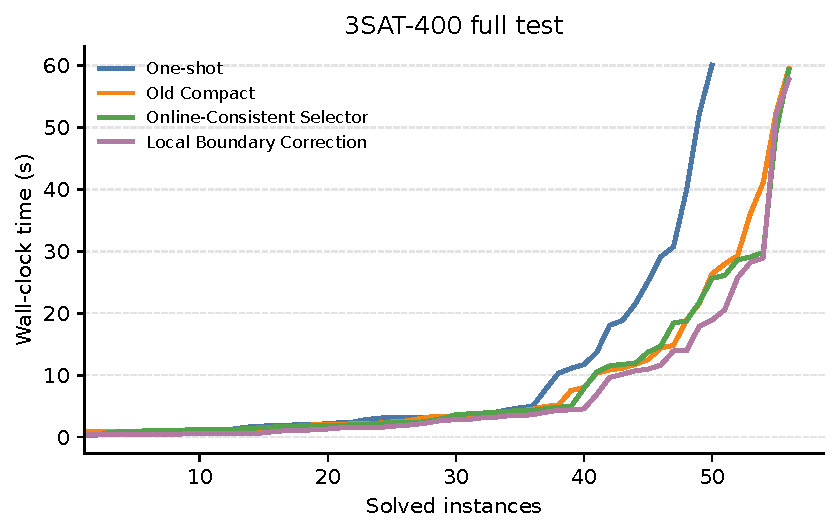
\includegraphics[width=0.78\linewidth]{fig_full400_cactus_paper.pdf}
\caption{Cactus plot over solved instances on the full 3SAT-400 test set. Curves sort solved instances by wall-clock solving time. Online-Consistent Selector preserves the timeout recovery of Old Compact while reducing mean time. Local Boundary Correction keeps the solved count unchanged and further reduces mean time by repairing a small set of guarded boundary cases.}
\label{fig:full400-cactus}
\end{figure}

\subsection{Instance-Level Behavior}

The full400 improvement is not uniform across all instances; it is concentrated in hard and timeout cases. Decision audits identify two important boundary classes. In \texttt{new\_opened\_old\_off} cases, the new selector opens an adapter branch that the old compact selector closed, such as \texttt{3sat\_140.cnf}, which drops from 41.083s to 4.339s. In \texttt{new\_closed\_old\_on} cases, the new selector closes a branch that earlier evidence opened. This includes correctly avoided slowdowns such as \texttt{3sat\_82.cnf}, but also over-conservative misses such as \texttt{3sat\_46.cnf} and \texttt{3sat\_196.cnf}. These boundary misses motivate the guarded Local Boundary Correction ablation.

\subsection{Stability Validation}

Stability validation uses only the final full400 per-instance results. We do not reuse old selector caches or retrain the main model. Table~\ref{tab:full400-stability} reports paired bootstrap and repeated split stability. Bootstrap uses 2000 paired resamples; repeated split samples 100 instances without replacement for 2000 trials.

\begin{table}[t]
\centering
\caption{Paired bootstrap and repeated split stability on the final full400 per-instance results. All deltas are measured against One-shot. Bootstrap uses 2000 paired resamples; repeated split samples 100 instances without replacement for 2000 trials.}
\label{tab:full400-stability}
\begin{tabular}{lrrrrr}
\toprule
Method & Solved & Mean time (s) & $\Delta$ mean (s) & Bootstrap 95\% CI & Split improve rate \\
\midrule
Old Compact & 56 & 46.348 & -1.403 & $[-2.729,\,-0.264]$ & 0.991 \\
Online-Consistent Selector & 56 & 46.222 & -1.530 & $[-2.823,\,-0.407]$ & 0.994 \\
+ Local Boundary Correction & 56 & 45.498 & -2.254 & $[-3.650,\,-1.068]$ & 1.000 \\
\bottomrule
\end{tabular}
\end{table}

The stability analysis supports the raw full400 interpretation. Online-Consistent Selector is a stable improvement over One-shot, while Local Boundary Correction mainly improves mean time rather than solved count.

\subsection{Local Boundary Correction Ablation}

Table~\ref{tab:boundary-ablation} summarizes the boundary correction ablations used in the paper narrative. The official full400 patch uses \texttt{intervention\_conflicts: [500, 750, 1000, 2000]} and the 750-feature decision rule. The no750 diagnostic opens a different neutral instance than the formal full400 patch and should not be mixed with the final full400 result.

\begin{table}[t]
\centering
\caption{Ablations used in the paper narrative. The official full400 boundary correction uses the 750-feature guarded rule. The no750 row is diagnostic only and has not replaced the official full400 patch.}
\label{tab:boundary-ablation}
\begin{tabular}{p{0.18\linewidth}p{0.22\linewidth}p{0.25\linewidth}p{0.25\linewidth}}
\toprule
Ablation & Scope & Result & Takeaway \\
\midrule
No guard & boundary subset & 5/26; mean 53.341 to 51.675 & Local signal exists, but needs a guard \\
Candidate guard & full400 & opens 4 candidates; 56/200; mean 45.498 & Guard keeps correction local \\
no750 diagnostic & trace only & opens 3 positive + 1 neutral & Diagnostic only; not official full400 patch \\
Local correction on/off & full400 & 56/200; mean 46.222 to 45.498 & Final boundary correction claim \\
\bottomrule
\end{tabular}
\end{table}

\subsection{Negative Results}

The negative results help explain why the paper does not continue adding selector complexity. Pairwise Veto improves over One-shot but reaches only 52/200 solved instances, below the Online-Consistent Selector. Compact Stable is useful as a failed stability branch, but it does not replace Old Compact as the reference baseline. Polarity and SBE variants are unstable on 3SAT-400 and are therefore kept out of the main method. These results support a conservative conclusion: the useful contribution is not a larger collection of gates, but an online-consistent selector with bounded local correction.

\section{Discussion and Limitations}

The experiments support a conservative interpretation. Neural feedback is not uniformly beneficial across all instances. It produces large gains on a small number of hard or timeout cases, but it can also introduce slowdowns or lost solutions. The Online-Consistent Selector is valuable because it makes adapter activation conditional on evidence from the actual CDCL trajectory, while keeping the final intervention sparse.

Local Boundary Correction exposes a remaining limitation: conservative risk control can close useful branches. The guarded correction repairs a small number of these boundary errors, but it is not a new global selector and does not increase solved count on full400. The official boundary correction uses the 750-feature guarded rule; no750 remains a diagnostic feature ablation.

The current evidence is strongest on the full 3SAT-400 test set. Appendix results on 3SAT-300 and 3SAT-350 show that the Online-Consistent Selector does not collapse on smaller held-out sizes, but these are generality checks rather than a new cross-scale claim. The repeated runtime audit is also scoped: it repeats fixed key instances under the same solver seed and therefore supports wall-clock stability of the key claims, not seed sensitivity.

\section{Conclusion}

This paper studies event-conditioned neural SAT guidance as a conservative intervention problem. Rather than calling a neural model at every branching decision, the solver collects low-frequency CDCL event traces, uses an Online-Consistent Selector to decide whether event-adapted guidance should be activated, and optionally applies a guarded Local Boundary Correction for a narrow class of over-conservative boundary cases. On held-out 3SAT-400 instances, this approach improves the one-shot neural guidance baseline from 50/200 to 56/200 solved instances and reduces mean wall-clock time. The results suggest that solver feedback is most useful when treated as sparse evidence for risk-controlled activation, not as an unconditional replacement for the baseline solver path.

\clearpage
\appendix

\section{Repeated Runtime Audit}

Table~\ref{tab:repeated-runtime-audit} reports the scoped same-seed repeated runtime audit. This audit repeats only the fixed key instances and does not test seed sensitivity. It supports all six recovered timeouts. \texttt{3sat\_196.cnf} and \texttt{3sat\_46.cnf} are stable hard speedups, \texttt{3sat\_188.cnf} is boundary-sensitive, and \texttt{3sat\_66.cnf} remains neutral timeout evidence.

\begin{table}[h]
\centering
\caption{Same-seed repeated runtime audit for the key recovered-timeout and guarded boundary-correction claims.}
\label{tab:repeated-runtime-audit}
\begin{tabular}{llll}
\toprule
Instance & Comparison & Stable? & Interpretation \\
\midrule
\texttt{3sat\_163.cnf} & One-shot vs Online-Consistent Selector & yes & recovered timeout stable \\
\texttt{3sat\_188.cnf} & One-shot vs Online-Consistent Selector & yes & recovered timeout stable \\
\texttt{3sat\_189.cnf} & One-shot vs Online-Consistent Selector & yes & recovered timeout stable \\
\texttt{3sat\_85.cnf} & One-shot vs Online-Consistent Selector & yes & recovered timeout stable \\
\texttt{3sat\_89.cnf} & One-shot vs Online-Consistent Selector & yes & recovered timeout stable \\
\texttt{3sat\_97.cnf} & One-shot vs Online-Consistent Selector & yes & recovered timeout stable \\
\texttt{3sat\_188.cnf} & Online-Consistent Selector vs + Local Boundary Correction & mixed & boundary-sensitive \\
\texttt{3sat\_196.cnf} & Online-Consistent Selector vs + Local Boundary Correction & yes & stable hard speedup \\
\texttt{3sat\_46.cnf} & Online-Consistent Selector vs + Local Boundary Correction & yes & stable hard speedup \\
\texttt{3sat\_66.cnf} & Online-Consistent Selector vs + Local Boundary Correction & yes & neutral timeout evidence \\
\bottomrule
\end{tabular}
\end{table}

\section{300/350 Generality Check}

Table~\ref{tab:appendix-300350} reports the smaller-size appendix check. These runs compare only One-shot and Online-Consistent Selector; Local Boundary Correction is not applied to 300/350. The results show that the final selector preserves solved count on 300, solves one additional instance on 350, and reduces mean time on both sizes.

\begin{table}[h]
\centering
\caption{Appendix generality check on smaller held-out 3SAT sizes. Local Boundary Correction is not applied to 300/350.}
\label{tab:appendix-300350}
\begin{tabular}{llrrrr}
\toprule
Size & Method & Solved & Mean time (s) & Median time (s) & $\Delta$ mean vs. One-shot (s) \\
\midrule
300 & One-shot & 200 & 15.311 & 14.099 & 0.000 \\
300 & Online-Consistent Selector & 200 & 7.272 & 6.061 & -8.039 \\
350 & One-shot & 108 & 43.741 & 57.104 & 0.000 \\
350 & Online-Consistent Selector & 109 & 33.815 & 40.065 & -9.925 \\
\bottomrule
\end{tabular}
\end{table}

\section{Artifact Sources}

The main source documents for this draft are \texttt{docs/paper\_intro\_abstract\_draft.md}, \texttt{docs/paper\_method\_section\_draft.md}, \texttt{docs/paper\_experiment\_section\_draft.md}, \texttt{docs/paper\_related\_work\_outline.md}, and \texttt{docs/paper\_tables\_and\_figures.md}. The paper-ready cactus plot is \texttt{figures/fig\_full400\_cactus\_paper.pdf}. The reproducibility package is tracked in \texttt{docs/paper\_reproducibility.md} and \texttt{docs/paper\_artifact\_manifest.md}. Checkpoints remain external artifacts or Git LFS candidates.

\bibliographystyle{plain}
\bibliography{references}

\end{document}
